
\addcontentsline{toc}{section}{Appendix} % Remove this if you don't want the appendix included in the table of contents.
\appendix


\section{MATLAB Code} \label{sec:matlab_code}
\subsection{Part 2} 

% hvor denne rare metoden (under) kommer fra:
% - https://tex.stackexchange.com/questions/254044/caption-and-label-on-minted-code
% Tips og triks til 'minted' saken
% - https://no.sharelatex.com/learn/Code_Highlighting_with_minted
\lstinputlisting[caption={Matlab code showing how the PSD function was calculated},label={mat:5.2.a},language=Matlab]{Matlabkode/p2_init.m}

\subsection{Part 4}
\lstinputlisting[caption={Matlab code showing ...},label={mat:5.4.a},language=Matlab]{Matlabkode/p4_til_rapport.m}

\subsection{Part 5}
Matlab function Simulink block 
\lstinputlisting[caption={Matlab code showing ...},label= {mat:kalman_func},language=Matlab]{Matlabkode/Kalman_function.m}
\lstinputlisting{Matlabkode/part5.m}\label{mat:part5}

\newpage
\section{Simulink Diagram} \label{sec:simulink_diagrams}

\subsection{Part 1}
\begin{figure}[H]
    \begin{center}
    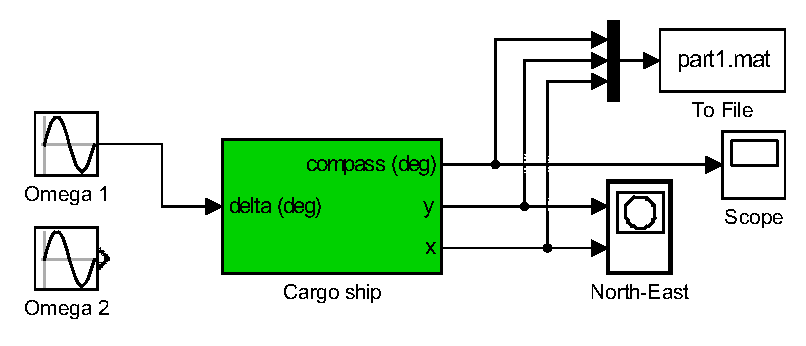
\includegraphics[width=1\linewidth]{Part1_pics/p5p1b.eps}
    \caption{System for part 1 b)}\label{sim:part1b}
    \end{center}
\end{figure}

\begin{figure}[H]
    \begin{center}
    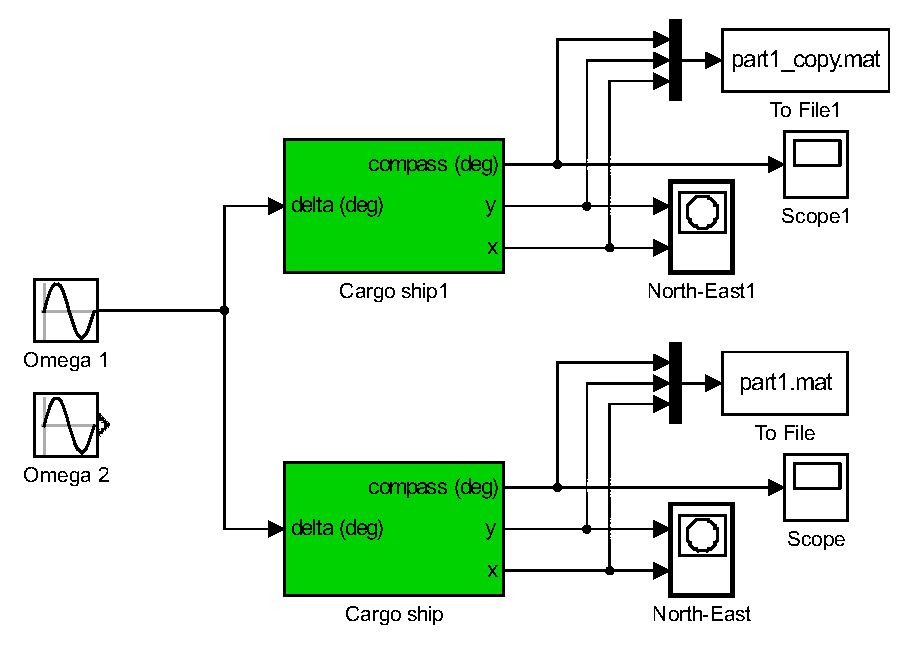
\includegraphics[width=1\linewidth]{Part1_pics/p5p1c.eps}
    \caption{System for part 1 c)}\label{sim:part1c}
    \end{center}
\end{figure}

\begin{figure}[H]
    \begin{center}
    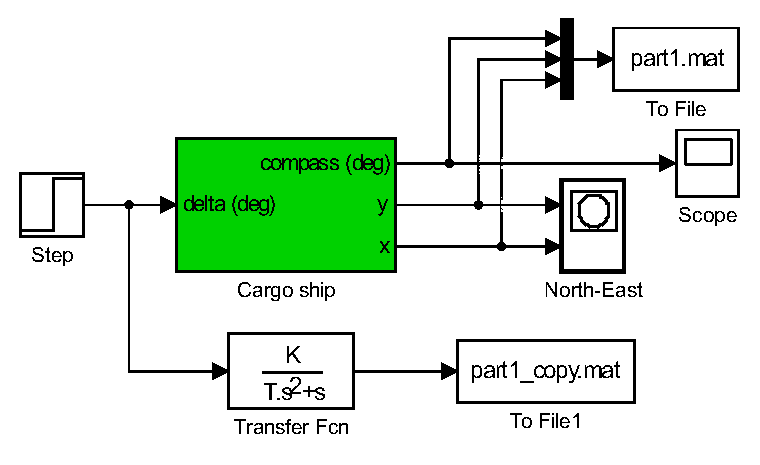
\includegraphics[width=1\linewidth]{Part1_pics/p5p1d.eps}
    \caption{System for part 1 d)}
    \label{sim:part1d}
    \end{center}
\end{figure}

\subsection{Part 2}
\begin{figure}[H]
    \begin{center}
    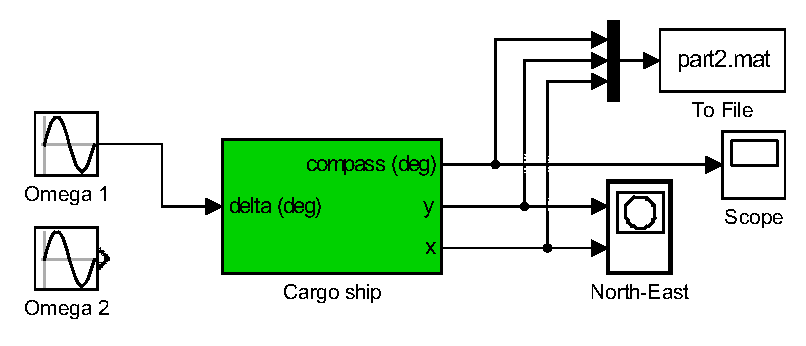
\includegraphics[width=1\linewidth]{Part2_pics/p5p2.eps}
    \caption{System for part 2}
    \label{sim:part2}
    \end{center}
\end{figure}

\subsection{Part 3}\label{sec:simulink_diagrams_3}
\begin{figure}[H]
    \begin{center}
    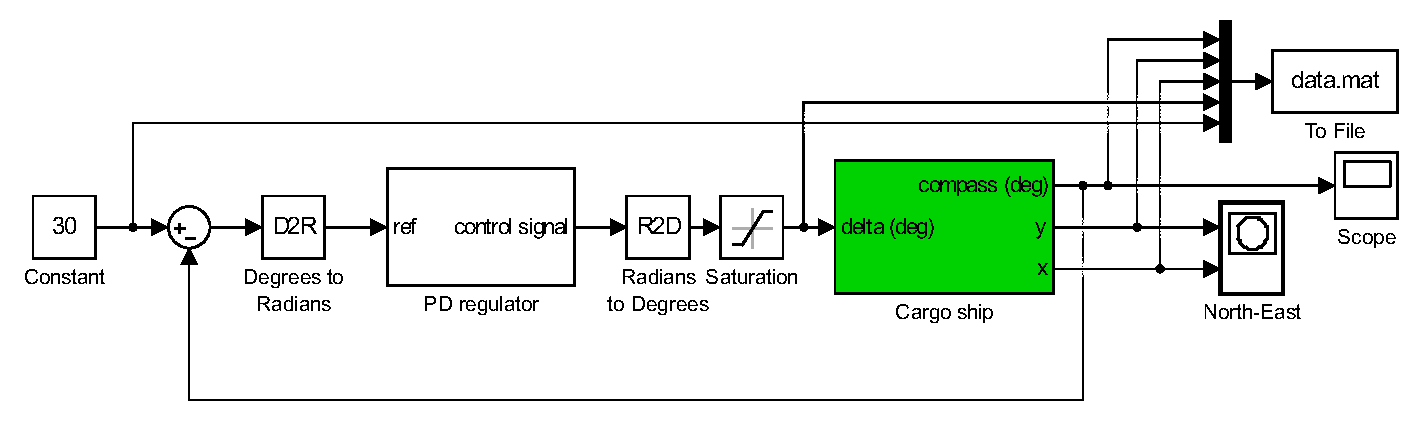
\includegraphics[width=1\linewidth]{Part3_pics/p5p3b.eps}
    \caption{System for part 3}\label{sim:part3}
    \end{center}
\end{figure}

\subsection{Part 5}
\begin{figure}[H]
    \begin{center}
    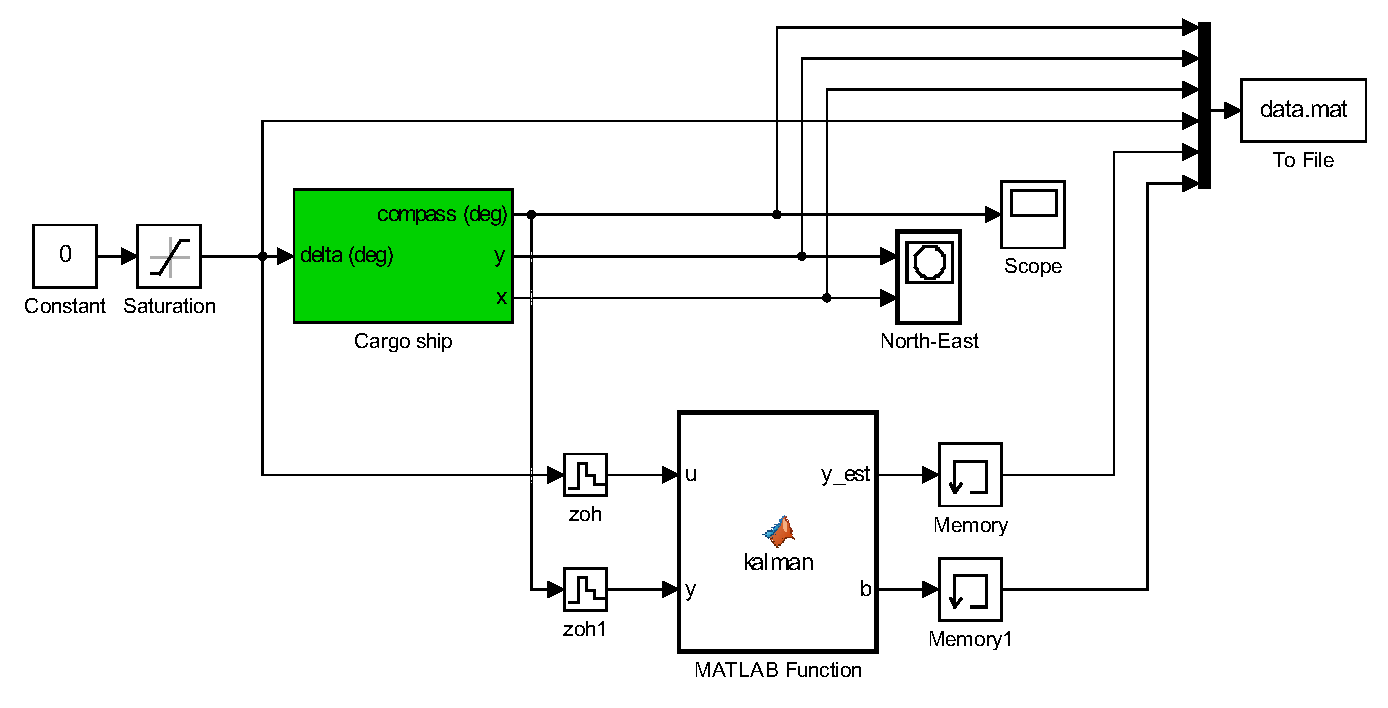
\includegraphics[width=1\linewidth]{Part5_pics/p5p5c.eps}
    \caption{System for part 5 c)}\label{sim:part5c}
    \end{center}
\end{figure}

\begin{figure}[H]
    \begin{center}
    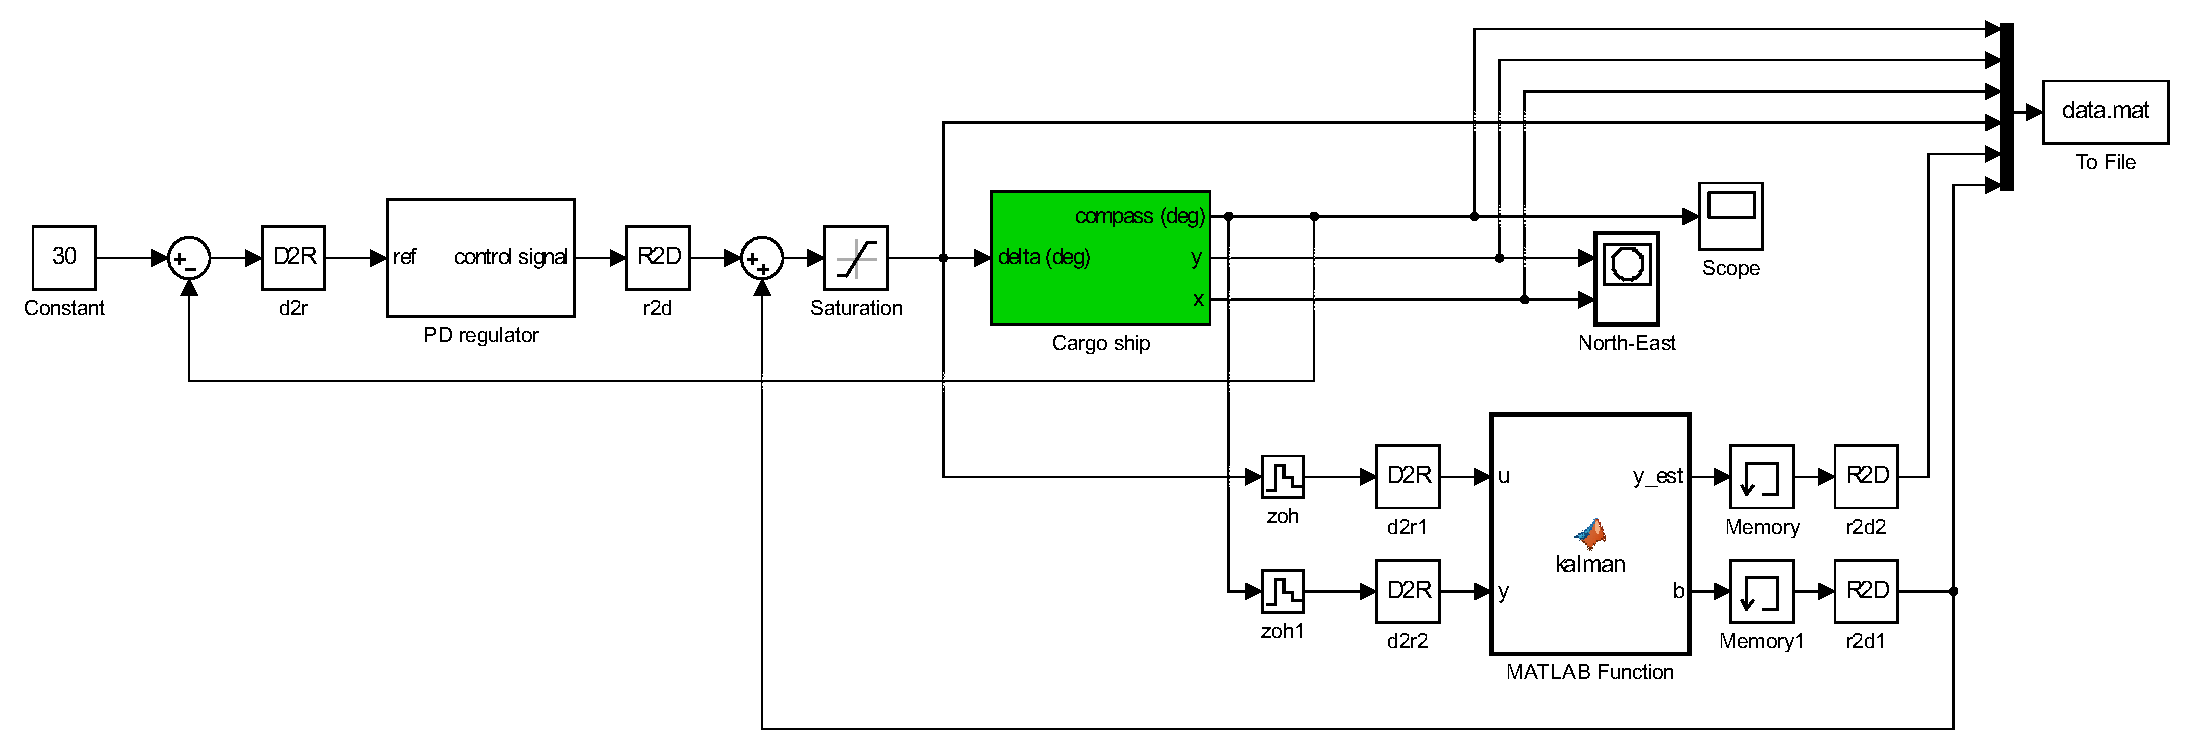
\includegraphics[width=1\linewidth]{Part5_pics/p5p5d.eps}
    \caption{System for part 5 d)}\label{sim:part5d}
    \end{center}
\end{figure}

\begin{figure}[H]
    \begin{center}
    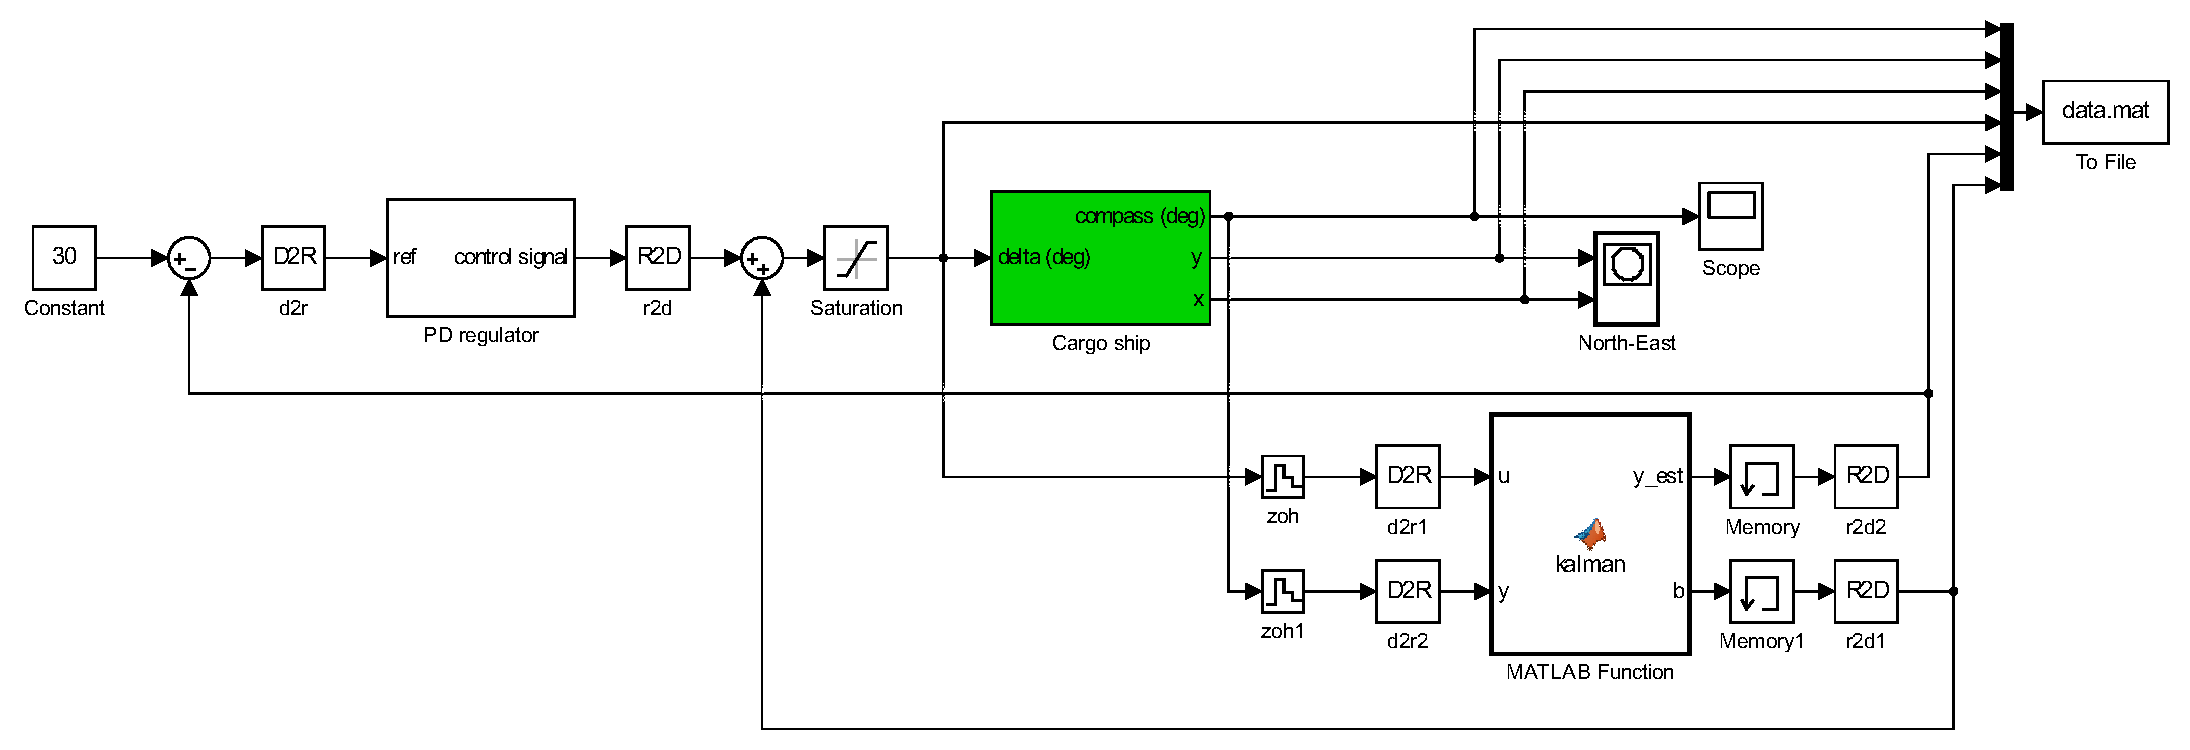
\includegraphics[width=1\linewidth]{Part5_pics/p5p5e.eps}
    \caption{System for part 5 e)}\label{sim:part5e}
    \end{center}
\end{figure}

\newpage
\section{Plots}

\subsection{Part 3}
\begin{figure}[H]
    \centering
    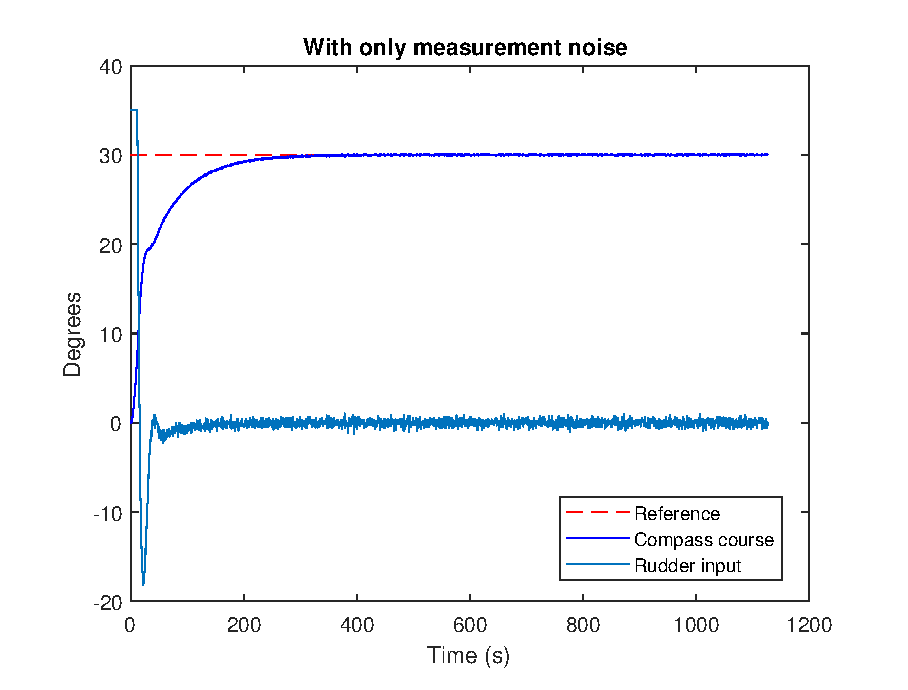
\includegraphics[width=1\linewidth]{Part3_pics/3b.eps}
    \caption{Compass compared to the reference}
    \label{sim:5.3.b}
\end{figure}
